\documentclass{./../../Latex/homework}
\begin{document}
\thispagestyle{plain}
\myheader{Homework 11 Solutions}

\subsection*{Exercise 11.5} 

%%%%%%% Question 1 (a)
\begin{enumerate}
\item (a) $ y = x^2 $
	
	Take two distinct points $x_1$ and $x_2$ and $0<\lambda<1$, then
	\begin{align}
	\begin{split}
		f\left(\lambda x_{1}+(1-\lambda) x_{2}\right) & =\left(\lambda x_{1}+(1-\lambda) x_{2}\right)^{2} \\
& =\lambda^{2} x_{1}^{2}+(1-\lambda)^{2} x_{2}^{2}+2 \lambda(1-\lambda) x_{1} x_{2}
\end{split}
\end{align}
Also note that, 
\begin{equation}
\lambda f\left(x_{1}\right)+(1-\lambda) f\left(x_{2}\right)=\lambda x_{1}^{2}+(1-\lambda) x_{2}^{2} 
\end{equation}

Subtracting (2) from (1)
$$  
\begin{aligned}
(1)-(2) &= \lambda^{2} x_{1}^{2}+(1-\lambda)^{2} x_{2}^{2}+2 \lambda(1-\lambda) x_{1} x_{2}-\lambda x_{1}^{2}-(1-\lambda) x_{2}^{2} \\
&= \lambda(\lambda-1) x_{1}^{2}-(1-\lambda) \lambda x_{2}^{2}+2 \lambda(1-\lambda) x_{1} x_{2} \\
&= \lambda(\lambda-1)\left(x_{1}^{2}+x_{2}^{2}-2 x_{1} x_{2}\right) \\
&= \lambda(\lambda-1)\left(x_{1}+x_{2}\right)^{2}<0 
\end{aligned}
  $$
Since $(1)-(2)<0$, 
$$ f\left(\lambda x_{1}+(1-\lambda) x_{2}\right)<\lambda f\left(x_{1}\right)+(1-\lambda) f\left(x_{2}\right)$$
So $f$ is strictly convex. \\

%%%%%%% Question 2 (c)
\item (c) $f(x,y) =xy$

Take two distinct points $u$ and $v$ and $0<\lambda<1$, then
	\begin{align}
	\begin{split}
		 f(\lambda u+(1-\lambda) v)&=f\left(\lambda u_{1}+(1-\lambda) v_{1}, \lambda u_{2}+(1-\lambda) v_{2}\right) \\
		 &=\left(\lambda u_{1}+(1-\lambda) v_{1}\right)\left(\lambda u_{2}+(1-\lambda) v_{2}\right) \\
&=\lambda^{2} u_{1} u_{2}+\lambda(1-\lambda) v_{1} u_{2}+\lambda(1-\lambda) u_{1} v_{2}+(1-\lambda)^{2} v_{1} v_{2}
\end{split}
\end{align}
Also note that, 
\begin{equation}
\lambda f(u)+(1-\lambda) f(v)=\lambda u_{1} u_{2}+(1-\lambda) v_{1} v_{2} 
\end{equation}

Subtracting (4) from (3)
$$  
\begin{aligned}
(4)-(3) = & \lambda(\lambda-1) u_{1} u_{2}+\lambda(1-\lambda) v_{1} u_{2}+\lambda(1-\lambda) u_{1} v_{2}-(1-\lambda) \lambda v_{1} v_{2} \\
= & \lambda(\lambda-1)\left[u_{1} u_{2}-v_{1} u_{2}-u_{1} v_{2}+v_{1} v_{2}\right] \\
= & \left.\lambda(\lambda-1)\left(\left(u_{1}-v_{1}\right) u_{2}-\left(u_{1}-v_{1}\right) v_{2}\right)\right] \\
= & \lambda(\lambda-1)\left(u_{1}-v_{1}\right)\left(u_{2}-v_{2}\right)
\end{aligned}
  $$
Since $(1)-(2)<0$, 
$$ f\left(\lambda x_{1}+(1-\lambda) x_{2}\right)<\lambda f\left(x_{1}\right)+(1-\lambda) f\left(x_{2}\right)$$
$f(.)$ is neither concave nor convex as (1) $\geq$ (2) sometimes and $(1) \leq(2)$ other times. \\

%%%%%%% Question 4
\item[4.] (a) No \hspace{1cm} (b) No \hspace{1cm} (c) Yes 

%%%%%%% Question 5
\item[5.] 
\begin{tasks}(2)
\task  
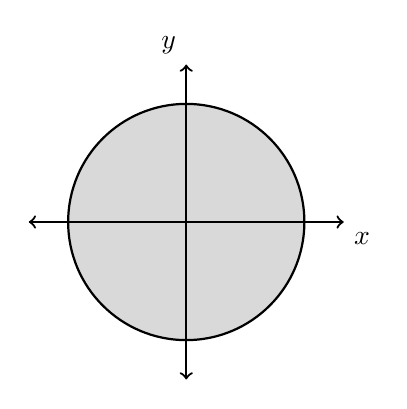
\begin{tikzpicture}[baseline=(current bounding box.north)] \draw[thick,fill=gray!30] (0,0) circle (1.5cm);
\draw[thick,<->] (-2,0) -- (2,0) node[anchor=north west] {$x$};
\draw[thick,<->] (0,-2) -- (0,2) node[anchor=south east] {$y$};

\end{tikzpicture}

\task Yes, convex. 
\end{tasks} 
\end{enumerate} 


\subsection*{Exercise 12.4} 

\begin{enumerate}
	
%%%%%%%% Question 1
\item Examples of acceptable curves:\\
\includegraphics[scale=0.5]{ex12.4q1.png}

%%%%%%%% Question 2
\item 
\begin{enumerate}
  \item $f(x) = a$ \\
Quasiconcave but not strictly so because for $u, v$ s.t $f(u) \geqslant f(v)$ :
$$
f(\lambda u+(1-\lambda) v)=f(v)=a
$$
\item $f(x)=a+b x \quad(b>0)$
\begin{tikzpicture}[baseline=(current bounding box.north)]
	% Draw axis     
    \draw[thick,->] (0,0) -- (6,0);
    \draw[thick,->] (0,0) -- (0,4);
    % Draw the function
    \draw[red, thick] (0,1) -- (5,3) node[anchor=south west] {};
    % Draw the dashed lines
    \draw[dashed] (2,0) -- (2,1.9);
    % Label points on the axes
    \node[anchor=north] at (2,0) {$u$};
    \node[anchor=east] at (0,1) {$a$};
    % Label the point v
    \draw[dashed] (4,0) -- (4,2.6);
    \node[anchor=north] at (4,0) {$v$};
\end{tikzpicture}


For any point between $u$ and $v$ given by $\lambda u+(1-\lambda) v$, the value of the function 
$f(\lambda u+(1-\lambda) v)$ will be strictly greater than $f(u)$ as $f$ is a strictly increasing function. So $f(.)$ is strictly quasiconcave.  
\item $f(x) = a+c x^2 \quad (c<0) $ 

To draw this function, let's calculate the first and the second derivatives:
$$ f^{\prime}(x)=2 c x, \quad \quad f^{\prime \prime}(x)=2 c<0 $$
Note that, for $f'(x)>0$ for $x<0$ and $f'(x)<0$ for $x>0$. Moreover, at $f(0) = a $. 

\begin{center}
\begin{tikzpicture}
    % Draw the axes
    \draw[thick,<->] (-4,0) -- (4,0);
    \draw[thick,<->] (0,-2) -- (0,4.25);
    % Draw the function
    \draw[red, thick, domain=-2.75:2.75, samples=100] plot ({\x}, {3.25 -0.5*\x*\x)});
    % Draw the dashed lines 
    \draw[dashed] (-1.6,0) -- (-1.6,2);
    \draw[dashed] (1,0) -- (1,2.75);
    % Label the points u, v, and a
    \node[anchor=north] at (-1.6,0) {$u$};
    \node[anchor=north] at (1,0) {$v$};
    \node[anchor=west] at (0,3.5) {$a$};
\end{tikzpicture}
\end{center}
From the graph of the function, we can see that this function is strictly quasiconcave.
\end{enumerate}

%%%%%%%% Question 4
\item [4.]
\begin{enumerate}
  \item $f(x)=x^{3}-2 x$ \\
  In the graph below, the blue line highlights the following upper-contour set:
  $$  S^U = \{x | f(x) \geq 0 \} $$
  We can see from the graph that this is not a convex set. So this function is not quasiconcave. Similarly, the lower-contour set for this function is not convex as well and this function is not quasiconvex. 
  \begin{center}
  	\includegraphics[scale=0.25]{desmos-graph.png}
  \end{center}

  \item $f\left(x_{1}, x_{2}\right)=6 x_{1}-9 x_{2}$
  
  Note that the upper-contour set for this function at 0:
   $$  S^U = \{(x_1,x_2) | 6 x_{1}-9 x_{2} \geq k \} $$
   Note that, $6 x_{1}-9 x_{2} = k \rightarrow x_2 = \frac{6x_1-k}{9}$.
So we can write the upper-contour set as:
   $$  S^U = \left\{(x_1,x_2) | x_2 \leq \frac{6x_1-k}{9} \right\} $$
   This set is presented below and is convex. Hence, the function is quasiconcave. The lower-contour set is also convex and the function is quasiconvex as well. (Grey is the upper-contour set and blue is the lower-contour set.)
  \begin{center}
  	\includegraphics[scale=0.25]{3b.png}
  \end{center}
  
  \item $f\left(x_{1}, x_{2}\right)=x_{2}-\ln x_{1}$ \\
  By similar reasoning as (b), this function is strictly quasiconcave but not quasiconvex. (Grey is the upper-contour set and blue is lower-contour set.) 
\end{enumerate}
  \begin{center}
  	\includegraphics[scale=0.25]{3c.png}
  \end{center}
\end{enumerate}

\subsection*{Exercise 12.6} 

%%%%%%%% Question 1
\begin{enumerate}
\item 
\begin{enumerate}
\item $f(x, y)=\sqrt{x y}$
$$
f(a x, a y)=\sqrt{(a x)(a y)}=\sqrt{a^{2} x y}=a \sqrt{x y}=a f(x, y)
$$
Homogeneous of degree 1 or linearly homogenous. 

\item
$$
\begin{aligned}
f(x, y) &=\left(x^{2}-y^{2}\right)^{1 / 2} \\
f(a x, a y) &=\left((a x)^{2}-(a y)^{2}\right)^{1 / 2} \\
&=\left(a^{2} x^{2}-a^{2} y^{2}\right)^{1 / 2} \\
&=\left(a^{2}\right)^{1 / 2}\left(x^{2}-y^{2}\right)^{1 / 2}=a f(x, y)
\end{aligned}
$$
Homogeneous of degree 1. 

\item $f(x, y)=x^{3}-x y+y^{3}$
$$
f(a x, a y)=a^{3} x^{3}-a^{2} x y+a^{3} y^{3}
$$
Not homogenous. 

\item Homogeneous of degree 1.
\item Homogeneous of degree 2.
\item Homogeneous of degree 4. 
\end{enumerate}

%%%%%%%% Question 2
\item Say we are given a production function $Q=f(K, L)$ that is homogenous of degree 1 or linearly homogenous. \\

Then dividing and multiplying by $K$ :

$$
Q=K \cdot \frac{Q}{K}=K \cdot f\left(\frac{K}{K}, \frac{L}{K}\right)=K \cdot f\left(1, \frac{L}{K}\right)=K \cdot \psi\left(\frac{L}{K}\right)
$$

Similarly, dividing and multiplying by $L$ :

$$
Q=L \cdot \frac{Q}{L}=L \cdot f\left(\frac{K}{L}, \frac{L}{L}\right)=L \cdot f\left(\frac{K}{L}, 1\right)=L \cdot \phi\left(\frac{K}{L}\right)
$$

\vspace{1em}

%%%%%%%% Question 6
\item[6.] $$Q=A K^{\alpha} L^{\beta}$$


(a) and (b) $$ f(a K, a L)=A(a K)^{\alpha}(a L)^{\beta}=A a^{(\alpha+\beta)} K^{\alpha} L^ \beta=a^{\alpha+\beta} f(K, L)$$

When $\alpha+\beta>1$, we have increasing returns to scale i.e. if we increase capital and labor by $a$-fold, output increases by more than $a$-fold. For eg. if we double $K$ and $L$, ie. $a=2, Q$ increases by $2^{\alpha+\beta}$, which is more than double when $\alpha+\beta>1$. Analogously, when $\alpha+\beta<1$, we have decreasing returns to scale, and when 
$\alpha+\beta=1$, we have constant returns to scale. \\

(c)
$$
 \begin{aligned}
\frac{d Q}{d K} &=\alpha A K^{\alpha-1} L^{\beta} \\
\frac{d Q}{d L} &=\beta A K^{\alpha} L^{\beta-1} \\
\varepsilon_{Q, K} &=\frac{d Q}{d K} \cdot \frac{K}{Q}=\frac{\alpha A K^{\alpha-1} L^ \beta}{A K^{\alpha} L^ \beta} \cdot K = \alpha\\
\varepsilon_{Q, L} &=\frac{d Q}{d L} \cdot \frac{L}{Q}=\frac{\beta A K^{\alpha} L^{\beta-1}}{A K^{\alpha} L^{\beta}} \cdot L =\beta
\end{aligned}
$$

\vspace{1em}

%%%%%%%% Question 7
\item[7.]  $$Q=A K^{a} L^{b} N^{c}$$

\begin{enumerate}

\item $f(d k, d L, d N)=d^{a+b+c} f(k, L, N)$. Homogeneous of degree $a+b+c$. 

\item  When $a+b+c=1$, constant returns to scale. When $a+b+c>0$, increasing returns to scale. 

\item  Marginal product of factor $N$:

$$Q_{N} =\frac{d Q}{d N}=c A K^{a} L^{b} N^{c-1} $$

If $N$ is paid it's marginal product, total payment to factor $N$ is $N \cdot Q_{N}$. So it's share in the output is given by:

$$ \frac{N \cdot Q_{N}}{Q} =N \cdot \frac{c A k^{a} L^{b} N^{c-1}}{A K^{a} L^{b} N^{c}}=c
$$
\end{enumerate}
\end{enumerate}


\end{document}